%%%%%%%%%%%%%%%%%%%%%%%%%%%%%%%%%%%%%%%%%%%%%%%%%%%%%%%%%%%%%%%%%%%%%%%%%%%%%%%%%%%%%
%%Universidade Federal de Uberlândia
%%Faculdade de Computação
%%Programa de Pós-graduação em Ciência da Computação
%%Plano de Trabalho
%%%%%%%%%%%%%%%%%%%%%%%%%%%%%%%%%%%%%%%%%%%%%%%%%%%%%%%%%%%%%%%%%%%%%%%%%%%%%%%%%%%%%%%

\documentclass[12pt]{article}
%\usepackage{sbc-template}
%\pagestyle{empty}
\textwidth 16cm \textheight 23.2cm
\voffset -1.5cm \hoffset -1.4cm

\usepackage[utf8]{inputenc}	
\usepackage[brazil]{babel}
\usepackage{graphicx,url}
\usepackage{subfigure}
\usepackage{enumitem}
\usepackage{amsfonts}
\usepackage{amsmath}
\usepackage{color}
\usepackage{physics}
\usepackage{comment}


\usepackage{lscape}

\usepackage{fancyhdr}


%\pagestyle{fancy}


\sloppy


\begin{document}
\rhead{\thepage}
\pagenumbering{arabic}

\begin{center}
	\bf{\LARGE{PROJETO DE DISSERTAÇÃO}\\ $\ $\\}
	\Large{Programa de Mestrado em Ciência da Computação\\
		Universidade Federal de Uberlândia}\\ $\ $\\
\end{center}

\begin{center}
	\bf{Aluno: Leandro Henrique Furtado Pinto Silva\\ $\ $\\
		Orientador: Prof. Dr. André Ricardo Backes\\ $\ $\\
		Coorientador: Prof. Dr. Maurício Cunha Escarpinati\\ $\ $\\
		Título do Trabalho: Detecção e Correção de distorções não-lineares para co-registro multiespectral de imagens agrícolas obtidas por veículos aéreos não tripulados.\\ $\ $\\
		Data de Início como Aluno Regular: agosto de 2019\\ $\ $\\
		Previsão da Defesa: agosto de 2021\\ $\ $\\}
\end{center}



\section{Introdução} 
\label{sec:introducao}

A humanidade, desde os primórdios, passou por um processo de crescimento populacional, sendo que esse ritmo se acelerou no último século. Prova disso é que estima-se que o número de habitantes do planeta há dois mil anos fosse próximo a 250 milhões. Em 1650, o número cresceu para 500 milhões. A marca de 1 bilhão de pessoas só foi atingida em 1850. O marco já tinha sido dobrado um século depois, quando, em 1950, a população era de aproximadamente 2,5 bilhões de pessoas \cite{Demografia2020}. Atualmente, a Organização das Nações Unidas (ONU) estima que a população global é cerca de 7,8 bilhões de pessoas \cite{UN2020}.

A obra de Thomas Robert Malthus, economista britânico, intitulada de ``\textit{Ensaio sobre o Princípio da População}'' (1798), que cunhou uma teoria bastante difundida na época, denominada de Teoria Malthusiana, era bastante pessimista. Malthus acreditava que a pobreza faria parte do destino da humanidade, baseando no pressuposto que a população humana possuía um potencial ilimitado de crescimento, ao contrário da produção de alimentos, a qual possuía limites. Malthus afirmava que enquanto a população crescia segundo uma progressão geométrica, a produção de alimentos crescia segundo uma progressão aritmética \cite{malthus1992malthus}. No final do século XIX diversos estudos também indicavam uma preocupação com o crescimento da população mundial e a capacidade do planeta de produzir alimentos. Esses estudos apontavam para um cenário futuro de escassez drástica de alimentos e, como consequência, à fome. 

As previsões não foram confirmadas, em grande parte devido aos significativos avanços tecnológicos que ocorreram na área agrícola nas décadas de 1950 e 1960. Um conjunto de iniciativas de desenvolvimento de tecnologias que possibilitaram aumentar a produção agrícola em todo o mundo, principalmente nos países em desenvolvimento. As iniciativas resultaram na adoção de novas tecnologias, incluindo variedades de cereais de alto rendimento, principalmente trigo e arroz, a utilização de fertilizantes químicos e agroquímicos, métodos de irrigação, novas formas de cultivo e a mecanização da lavoura \cite{malthus1872essay, hazell2009asian, farmer1986perspectives}. 

No Brasil, o setor do agronegócio mostra-se cada vez mais consolidado. Prova disso é que em meio a pandemia de SARS-CoV-2 (``\textit{novo coronavirus}''), declarada pela ONU em 11 de março de 2020, o setor do agronegócio foi o único a apresentar crescimento, segundo o Instituto Brasileiro de Geografia e Estatística (IBGE). O crescimento, embora tímido (cerca de 0,6\%), no primeiro trimestre de 2020, evidencia a força do setor, mesmo em um período traumático para a economia nacional e internacional. Ainda segundo o IBGE, se compararmos com o mesmo período de 2019, o setor do agronegócio teve crescimento de 1,9\%, indo na contramão dos indicadores gerais do país, onde houve queda no PIB de 1,5\% \cite{UNCovid,IBGE,IBGE2}.

Um dos principais componentes da fase atual das pesquisas agrícolas é a agricultura de precisão (AP), que pode ser caracterizada pela gestão agrícola baseado na observação, medição e resposta à variabilidade inter e intra-campo nas lavouras. O objetivo da pesquisa em AP é definir um Sistema de Suporte à Decisão para o gerenciamento de toda a fazenda, com o objetivo de otimizar o retorno dos insumos e preservar os recursos. A área de AP mostrou-se fortemente dependente das tecnologias de imagem e mapeamento para estimar o crescimento ou identificar outras características agronômicas importantes, como por exemplo o estresse por nitrogênio. Diante desse cenário, com a crescente importância da utilização de imagens na AP, alguns mecanismos de obtenção dessas imagens foram se destacando, em especial, os Veículos Aéreos Não Tripulados (VANTs).


Os avanços na tecnologia VANTs, especialmente na última década, levaram à sua ampla divulgação nos mais diversos seguimentos, incluindo a agricultura de precisão. Com a consequente redução dos custos de produção e a queda nos custos operacionais, pequenos e médios produtores agora podem pagar o uso de tecnologias auxiliadas por imagem, como os VANTs \cite{jenkins2013economic}. 


Diferente de outros dispositivos de aquisição de imagens aéreas, como satélites e grandes aeronaves, os VANTs permitem capturar imagens em altitudes baixas e médias (50 a 400 m), proporcionando uma visão mais detalhada da região analisada. Outro elemento importante para a eficácia das análises realizadas com este equipamento são os sensores utilizados. Existe uma grande variedade de dispositivos usados no processo: câmeras RGB, sensores de captura de calor, câmeras multi e hiperespectrais, entre outros. Cada dispositivo possui características próprias e produz informações que exigem a diferentes tipos de análises. No entanto, o processo de aquisição de dados, em geral, é o mesmo independente do sensor utilizado: o equipamento é acoplado à aeronave e as imagens são capturadas sequencialmente durante o voo. Após o término do processo, essas imagens são organizadas em mosaico capaz representar toda a área \cite{mcbratney2005future,milella2019multi,blackmer1996aerial,sankaran2015low,kataoka2003crop}. 

Uma imagem multi ou hiperespectral, para ser útil em aplicações agrícolas, necessita, primeiramente, ter suas bandas alinhadas. Esse processo, o qual é conhecido como co-registro de banda, apresenta uma série de dificuldades para ser realizado \cite{junior2019detection}. 

A primeira dificuldade a se considerar é fato de cada elemento presente na imagem estar representado de forma diferente em cada espectro, em virtude de características químicas e físicas. Processos de emissão, absorção, reflexão e transmissão variam para cada um dos espectros. Diante disso, há perda de informação e, consequente, dificuldade no processo de alinhamento \cite{banerjee2018alignment}.

Outro fator é que a maioria das câmeras multiespectral utiliza de sensores distintos para obtenção dos espectros. Em outras palavras, mesmo se a câmera for colocada em uma plataforma fixa, apenas o deslocamento físico entre os sensores já é responsável por causar o desalinhamento entre as bandas (canais). Entretanto, quando acoplado ao VANT, o problema se intensifica. O voo do VANT está sujeito, por exemplo, a vários fatores: velocidade do VANT, velocidade do vento, subidas e descidas do VANT, condições meteorológicas do ambiente e outros \cite{junior2019detection, banerjee2018alignment}. 

Há ainda diversas deformações que podem ser observadas em imagens capturadas por VANTs na Agricultura de Precisão. Dentre essas deformações, estão variações lineares (rotação, translação e escala, por exemplo) e não-lineares (as quais possuem características variadas e sem um padrão previamente definido). Assim, é necessário identificar e corrigir as distorções presentes para que se possa extrair o maior valor das imagens capturadas durante o voo.

Na literatura, o trabalho de \cite{dias2020uav} contribuiu significativamente com a caracterização do problema de desalinhamento entre canais de uma imagem obtida por VANT na AP. Entretanto, \cite{dias2020uav} considera apenas deformações lineares. Por outro lado, o trabalho de \cite{eppenhof2019progressively} propõe o tratamento de deformações não lineares para o problema de registro. Mas, \cite{eppenhof2019progressively} trabalha com imagens de tomografias pulmonares. Assim, a contribuição do trabalho se dará em tratar deformações não lineares em imagens multiespectrais de VANTs na AP.

O presente projeto está dividido da seguinte forma: a seguir serão apresentados Objetivos e Justificativa. Na seção \ref{sec:literatura} apresentamos a revisão da literatura correlata; já a seção \ref{sec:trab_relacionados} apresenta os trabalhos relacionados, os quais serão suporte para o desenvolvimento deste. Por fim, as seções \ref{sec:metodologia}, \ref{sec:resultados} e \ref{sec:cronograma} discorrem, respectivamente, sobre a metodologia a ser desenvolvida, resultados esperados e cronograma de execução.

\subsection{Objetivos}

\label{sec:objetivos}

O objetivo deste projeto é realizar o co-registro entre bandas de imagens obtidas por VANTs, especificamente em agricultura de precisão. Deste modo, desenvolver métodos para detecção e correção de distorções \textbf{não-lineares} geradas durante o processo de aquisição por conta de forças externas que interferem no voo do VANT. 

Mais especificamente, tem-se por objetivos:
\begin{enumerate}
    \item Avaliar técnicas para tratamento de distorções não lineares entre os canais de uma imagem.
    \item Investigar a eficiência de métodos de algoritmos inteligentes, baseado em \textit{deep learning}, para estimar o grau de distorções não lineares entre os canais de uma imagem multiespectral.
    \item Realizar, a partir da estimativa do grau de distorção, o registro entre as bandas\footnote{Também chamado de co-registro.} de uma imagem.
    \item Analisar e avaliar os resultados das melhorias em relação ao estado da arte para o problema.
\end{enumerate}

\subsection{Justificativa}
\label{sec:justificativa}

Ainda que o processo de aquisição de imagens multiespectrais, especialmente em baixa/média altitude, tenha se tornado mais simples, o desafio de alinhar as diferentes bandas, especialmente quando há deformações não lineares, se caracteriza como um grande desafio.

A situação supracitada acontece pelo simples fato das técnicas atuais serem consolidadas e robustas em problemas de processamento de imagens mais estáveis e com uma cobertura espacial maior quando comparados com aquelas obtidas por VANTs \cite{PANTANO, sensores2, sensores}. Conforme mencionado, as imagens que são objetos de estudo do trabalho são de natureza multi espectral. Em outras palavras, cada banda cobre uma faixa diferente do espectro eletromagnético (veja Figura \ref{fig:espectro_eletromagnetico}). Desta forma, pode acontecer de objetos que são representados por um espectro não ser representado em outros. Tal situação prejudica a tarefa de encontro de pontos de controle e torna a tarefa mais complexa, quando temos imagens deste nicho. Além disso, a complexidade da tarefa ainda aumenta consideravelmente quando temos distorções entre essas bandas, especialmente as não lineares \cite{dias2020uav, junior2019detection}.

\begin{figure}[!ht]
    \centering
    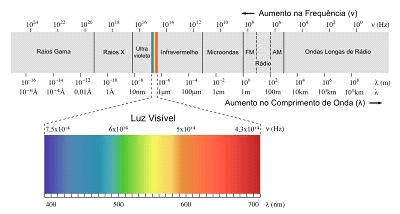
\includegraphics[width=0.6\textheight]{figures/espectro_eletromagnetico.png}
    \caption{Representação do Espectro Eletromagnético \cite{da2015light}.}
    \label{fig:espectro_eletromagnetico}
\end{figure}


A Figura \ref{fig:espectros} apresenta as cinco bandas separadas de uma mesma imagem capturada por VANT em um uma plantação de soja. Posteriormente, a Figura \ref{fig:desalinhamento} apresenta uma imagem composta por dois espectros, através de \textit{checkerboard} (onde tons claros e escuros diferenciam distintos espectros). Nessa Figura é possível enxergar o desalinhamento entre os espectros de uma mesma imagem. Em outras palavras, a simples sobreposição das bandas representaria uma imagem multiespectral completamente desalinhada.  


\begin{figure}[!ht]
    \centering
    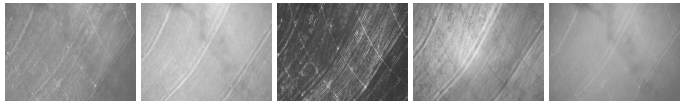
\includegraphics[width=0.6\textheight]{figures/espectros.png}
    \caption{Exemplo de uma imagem contendo todas as bandas. Azul, Verde, Vermelho, Infravermelho Próximo e Infravermelho, respectivamente \cite{dias2020uav}.}
    \label{fig:espectros}
\end{figure}

\begin{figure}[!ht]
    \centering
    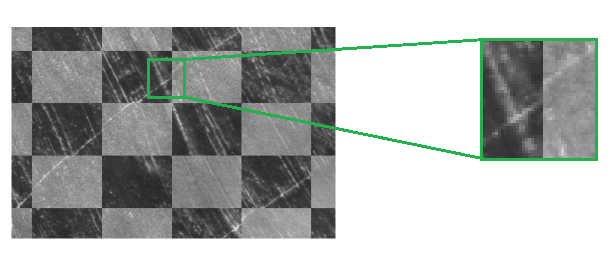
\includegraphics[width=0.6\textheight]{figures/visualiza_desalinhamento.png}
    \caption{\textit{Checkerboard} de dois canais de uma mesma imagem \cite{dias2020uav}.}
    \label{fig:desalinhamento}
\end{figure}


Além disso, a utilização de VANTs para obtenção de imagens agrícolas demanda por centenas ou, em muitos casos, milhares de sobreposições para cobrir uma determinada área, o que demanda consideravelmente por técnicas robustas para alinhar as bandas de cada uma dessas imagens.


\section{Revisão da Literatura Correlata} 
\label{sec:literatura}


\subsection{Sensoriamento Remoto na Agricultura de Precisão}

O sensoriamento remoto pode ser definido como a obtenção de informação sobre um determinado objeto sem o contato físico. Na AP, especificamente, consiste em um processo de captura de dados em nível de campo. Inicialmente, as imagens eram obtidas por satélites, aviões ou helicópteros \cite{zarco2016new}. Entretanto, esses processos não forneciam dados com rapidez suficiente para o uso considerado ``ideal'' dos métodos de PA. Além disso, eram consideravelmente caros. 

Por outro lado, principalmente na última década, o desenvolvimento e popularização dos VANTs fomentou uma nova era da AP. Esses equipamentos têm a capacidade de fornecimento de dados de resolução espacial, espectral e temporal sem precedentes \cite{maes2019perspectives, dyrmann2016plant}.

Na AP, as imagens de sensoriamento remoto possuem os mais variados usos: classificação de espécies de culturas, monitoramento de doenças e ervas daninhas, detecção de estresse hídrico e mapeamento de propriedades do solo \cite{ihuoma2017recent}. Entretanto, alguns aspectos precisam ser avaliados antes de utilizar as imagens de sensoriamento remoto para o processos de tomadas de decisão. Vários parâmetros são afetados pelo tipo de plataforma (satélite, aérea ou terrestre) e pelo sensor escolhido para a aquisição dos dados: (1) precisão geométrica das imagens; (2) radiométrico; (3) espectral; (4) espacial; (5) resolução temporal; (6) largura e o número de bandas espectrais; (7) qualidade da informação espectral representada nas imagens \cite{khanal2017overview}. 

\begin{figure}[!htpb]
    \centering
    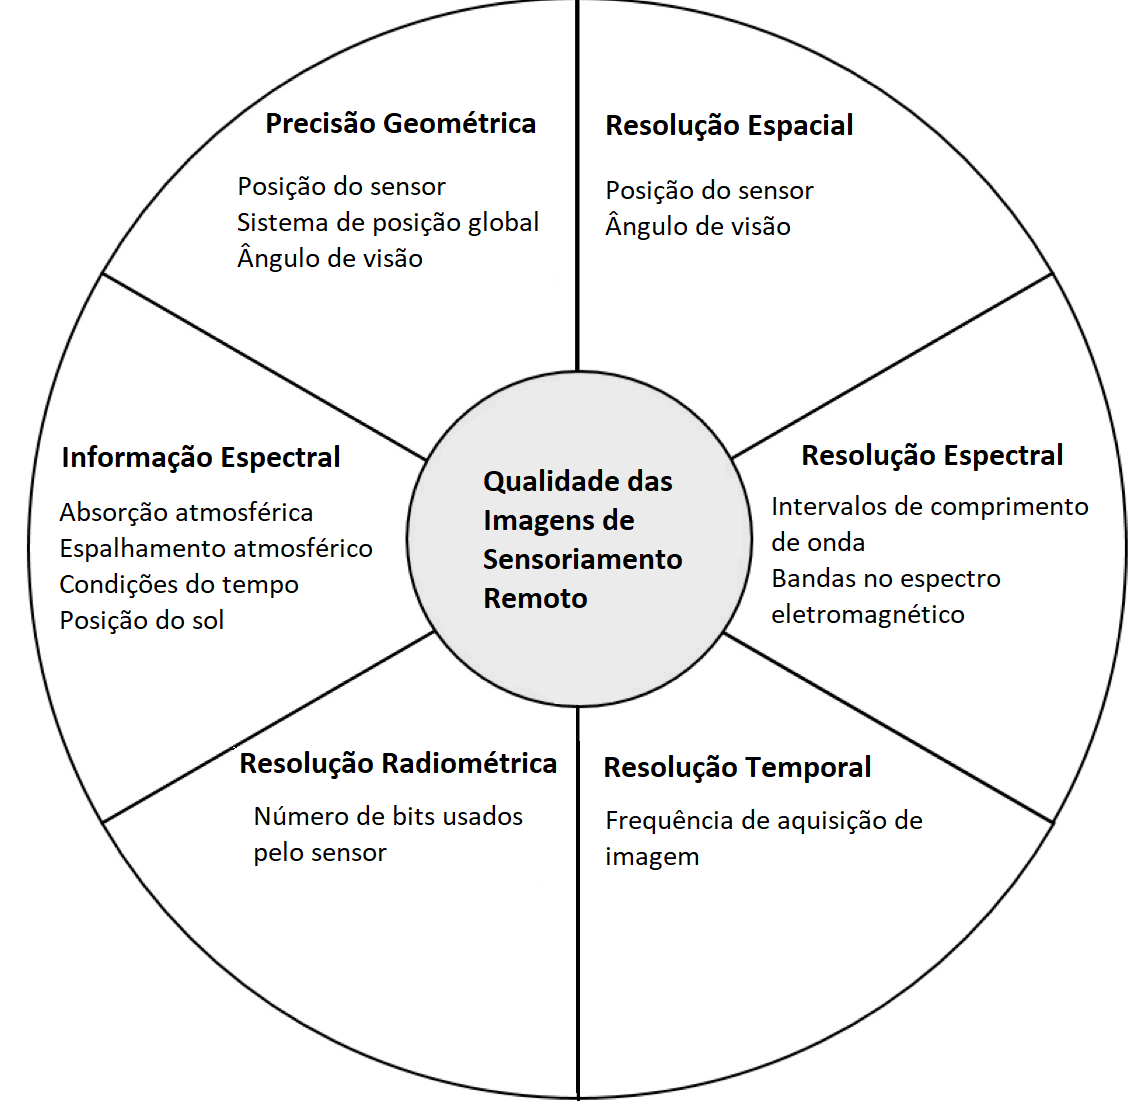
\includegraphics[width=0.5\textheight]{figures/qualidade_imagens.png}
    \caption{Fatores de qualidade em sensoriamento remoto \cite{khanal2017overview}.}
    \label{fig:qualidade_imagens}
\end{figure}


\subsection{Redes Neurais Artificiais}

As Redes Neurais são sistemas computacionais concebidos com base no estudo do cérebro humano. Assim, as Redes Neurais se diferenciam dos demais modelos computacionais existentes. Tal diferenciação deve-se pelo fato do paradigma neural não fazer uso dos conceitos que até então caracterizavam os demais algoritmos de sistemas computacionais \cite{thome2002redes}.

Os modelos neurais nasceram baseando-se na estrutura do sistema nervoso, especificamente na estrutura do cérebro humano. Diante disso, sua principal característica está na capacidade de aprender baseando-se na exposição de exemplos. Assim, a construção de uma rede neural baseia-se na configuração da sua arquitetura interna (uma rede interligada de neurônios) e no treinamento da referida rede, baseando-se em exemplos, a fim de que a própria consiga aprender como resolver os problemas \cite{thome2002redes}.

Em sua tarefa de simular a estrutura de funcionamento básico do cérebro, as redes neurais utilizam um modelo matemático (abstrato) do neurônio cerebral. Nesse sentido, a intensidade das ligações entre neurônios são emuladas através de pesos, que são ajustáveis durante o processo de evolução do treinamento da rede. O corpo celular é emulado através da composição de duas funções: ativação e propagação. O objetivo dessas funções é mapear os sinais de entrada em um único sinal de saída. Tal sinal de saída será então propagado para os neurônios seguintes da rede, tal como um modelo biológico.

\subsubsection{O Modelo Neural}

Há diversos modelos de redes neurais expostos na literatura. Cada um desses modelos advém de diferentes linhas de pesquisa e visam um melhor desempenho na solução de um problema em específico \cite{fausett2006fundamentals}. Basicamente, os modelos neurais podem ser classificados como:

\begin{itemize}
    \item \textbf{A Estratégia de treinamento:} (1) supervisionadas, onde a rede dispõe de um instrutor apontando acertos e erros; ou (2) não supervisionadas, no caso contrário a (1).
    \item \textbf{A forma de treinamento:} (1) incremental, o qual ocorre quando o conhecimento se ajusta após a apresentação de cada padrão de entrada; ou (2) em lote, quando o ajuste do conhecimento só será realizado após a ``visão'' de todos os estímulos.
    \item \textbf{A forma de operação:} (1) unidirecional, onde os sinais internos se propagarão apenas na direção entrada/saída; ou (2) recorrente, quando houver a realimentação do referido processo.
\end{itemize}


\subsubsection{\textit{Multi Layer Perceptron}}

Um neurônio artificial consiste na unidade fundamental para processamento de informações de uma rede neural artificial. O modelo matemático de um neurônio artificial foi concebido pelos pesquisadores W. S. McCulloch e W. H. Pitts, em 1943. Tal modelo, é composto, basicamente, de conexões simulando os dendritos, pesos simulando as sinapses, uma função de mapeamento simulando o corpo celular, além de uma saída que simula o axônio \cite{fausett2006fundamentals}. A Figura \ref{fig:neuronio} ilustra a o modelo matemático de um neurônio artificial.

\begin{figure}[!ht]
    \centering
    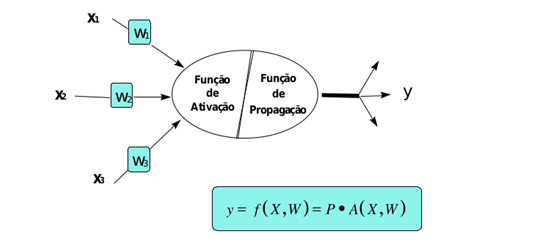
\includegraphics[width = 0.65\textheight]{figures/neuronio.png}
    \caption{O modelo matemático de um neurônio artificial \cite{thome2002redes}.}
    \label{fig:neuronio}
\end{figure}

Neste sentido, o Perceptron é um algoritmo para aprendizado de classificações binárias. O Perceptron possui a capacidade de resolver problemas linearmente separáveis, através do processo de treinamento, o qual o algoritmo aprende a classificar a entrada em dois grupos diferentes.

Para tratarmos de problema não linearmente separáveis, podemos fazer uso de um Perceptron Multicamadas (MLP - \textit{Multi Layer Perceptron}). Em uma MLP o aprendizado é, geralmente, feito por intermédio do algoritmo de retropropagação do erro. Em suma, a fim de treinarmos uma rede neural por intermédio de retropropagação do erro, envolveremos três estágios: (1) o \textit{feedforward} do padrão de treinamento, (2) o cálculo e a retroprogagação do erro associado e, por fim, (3) o ajuste dos pesos. Segundo Fausett (1993), após o treinamento, a solução da rede se dá pelo cálculo da fase de \textit{feedfoward} \cite{fausett2006fundamentals}.

\subsubsection{A Estrutura de uma Rede Neural}

A construção de uma rede neural baseia-se na configuração da sua arquitetura interna (uma rede interligada de neurônios) e no treinamento da referida rede, baseando-se em exemplos, a fim de que a própria consiga aprender como resolver os problemas \cite{hassoun1995fundamentals}.

Geralmente, uma rede neural é organizada em uma estrutura de camadas com um padrão de conexão completa inter-camadas, apenas na direção entrada/saída e nenhuma conexão intra-camada. Em outras palavras, um neurônio situado em uma determinada camada possui sua saída conectada a todos os neurônios da camada seguinte e a nenhum outro de qualquer outra camada \cite{hassoun1995fundamentals}. A Figura \ref{fig:rede_neural} ilustra a estrutura topológica mencionada.

\begin{figure}[!ht]
    \centering
    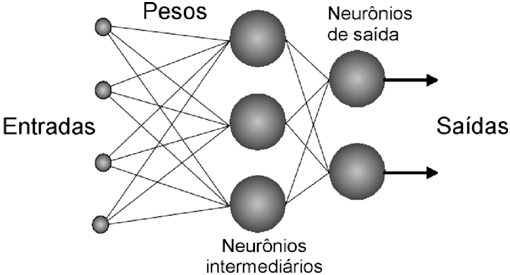
\includegraphics[width=0.6\textheight]{figures/EstruturaRedeNeural.png}
    \caption{Estrutura de uma Rede Neural \cite{daalvaro}.}
    \label{fig:rede_neural}
\end{figure}


\subsection{Redes Neurais Convolucionais}

As Redes Neurais Convolucionais (CNNs, do inglês \textit{Convolutional Neural Networks}) são uma categoria de algoritmos de aprendizado profundo, inspiradas processo de aprendizado humano. Essas redes são baseadas no conceito de campo receptivo de sistemas biológicos, o que dá a essas redes a capacidade de aprender diferentes filtros e características de uma imagem. Dessa forma, a CNN pode explorar as correlações espaciais entre \textit{pixels} em uma imagem para extrair atributos de imagem relevantes para diferentes tarefas, como classificação e segmentação de imagens \cite{Lecun1998,Guo2016,Ponti2017}.

A maioria dos modelos de CNN disponíveis na literatura é definida em termos de três tipos de camadas (convolucional, de \textit{pooling} e densa), as quais são combinadas de maneira diferentes para melhorar a classificação ou segmentação da imagem.

A camada convolucional é responsável por extrair atributos significativos de uma imagem. Para isso, aplica-se uma série de operações de convolução sobre os dados de entrada, que atuam como filtros receptivos e, desta forma, se destacam diferentes atributos de uma região local da imagem. Uma função de ativação \textit{ReLU} (\textit{REctified Linear Unit}) e, geralmente, uma operação de \textit{Normalização de Lote}, a depender da arquitetura em questão, são aplicadas ao resultado da camada convolucional. Isso ajuda a acelerar o treinamento da rede e a melhorar seus resultados \cite{LeCun2015}.

As camadas convolucionais são geralmente seguidas por uma camada de \textit{pooling}, cujo objetivo é reduzir os mapas de características calculados pelas camadas anteriores, reduzindo assim a sensibilidade da rede a distorções na imagem e na mudança de dados. Em geral, é usada uma máscara de tamanho $2 \times 2$, reduzindo assim uma região de 4 \textit{pixels} para um valor único de acordo com algum critério (por exemplo, pixel máximo ou médio da região) \cite{Scherer2010}.

No final da CNN, encontramos as camadas densas. Cerca de 90\% dos parâmetros de uma CNN são encontrados nessas camadas. Essas camadas recebem como entrada os mapas de características 2D obtidos das camadas anteriores, com o objetivo de aprender um vetor de características 1D capaz de discriminar a imagem de entrada. Esse vetor é usado como entrada de um classificador \textit{softmax}, que retorna a classe mais provável para uma determinada imagem de entrada.

\subsection{Redes Neurais Convolucionais Siamesas}

Redes siamesas são redes neurais que contém dois ou mais componentes de sub-redes totalmente idênticos. As entradas de uma rede siamesa podem ser dados numéricos, dados de imagem ou mesmo dados sequenciais, tais como sentenças ou sinais de tempo. A característica principal das redes siamesas é o fato de poderem aprender descritores de dados úteis, relacionados com as entradas fornecidas em cada sub-rede. Esses descritores podem utilizados para efeitos de comparação dentre as entradas das respectivas sub-redes \cite{bromley1994signature}. Um exemplo de modelo de uma rede siamesa pode ser ilustrada conforme a Figura \ref{fig:siameseCNN}

\begin{figure}[!ht]
    \centering
    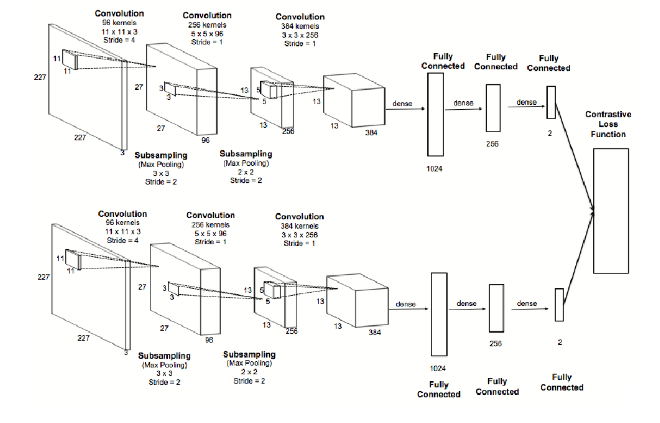
\includegraphics[width = 1\textwidth]{figures/siameseCNN.png}
    \caption{Exemplo de uma rede neural convolucional siamesa. Fonte: \cite{rao2016deep}.}
    \label{fig:siameseCNN}
\end{figure}

Geralmente, as redes siamesas realizam classificação binária na saída, ou, em outras palavras, classificam se as entradas são da mesma classe ou não \cite{rao2016deep}. Dessa forma, diferentes funções de perda podem ser utilizadas durante o treinamento. Uma das funções de perda mais populares é a \textit{Binary Cross-Entropy Loss}, a qual pode ser calculada de acordo com a Equação \ref{equation1}:

\begin{equation}
    L = -y \ log \ p + (1 - y) \ log \ (1 - p)
    \label{equation1}
\end{equation}

\noindent onde $L$ é a função de perda, $y$ é o rótulo da classe (0 ou 1) e $p$ é a previsão. Para treinar a rede, a fim de diferenciar entre objetos semelhantes e diferentes, podemos fornecer um exemplo positivo e um negativo por vez e somar as perdas, conforme Equação \ref{equation2}:

\begin{equation}
    L = L_+ + L_-
    \label{equation2}
\end{equation}


\subsection{U-Net}

A U-Net é uma arquitetura inspirada na \textit{Fully Convolutional Network}, proposta por \cite{long2015fully} para tratar problemas de segmentação em imagens médicas (veja a Figura \ref{fig:exemplo_unet}).

\begin{figure}[!ht]
    \centering
    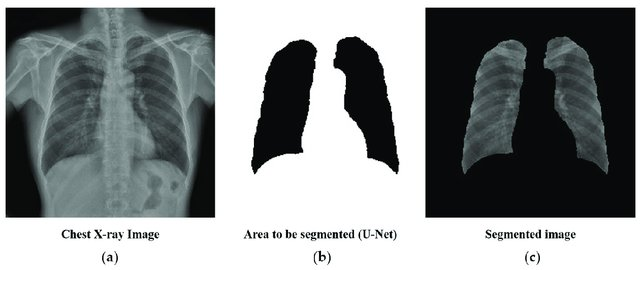
\includegraphics[width = 0.6\textheight]{figures/exemplo_unet.png}
    \caption{Segmentação pulmonar antes e após o treinamento com uma U-Net. Fonte: \cite{heo2019deep}.}
    \label{fig:exemplo_unet}
\end{figure}

A ideia principal da U-Net consiste em substituir as operações de \textit{pooling} por operações de \textit{upsampling}. Dessa forma, essas camadas conseguem aumentar a resolução de saída. Além disso, a utilização de uma camada convolucional sucessiva pode conseguir aprender a montar uma saída precisa, com base nas informações de entrada \cite{unet}.


\begin{figure}[!ht]
    \centering
    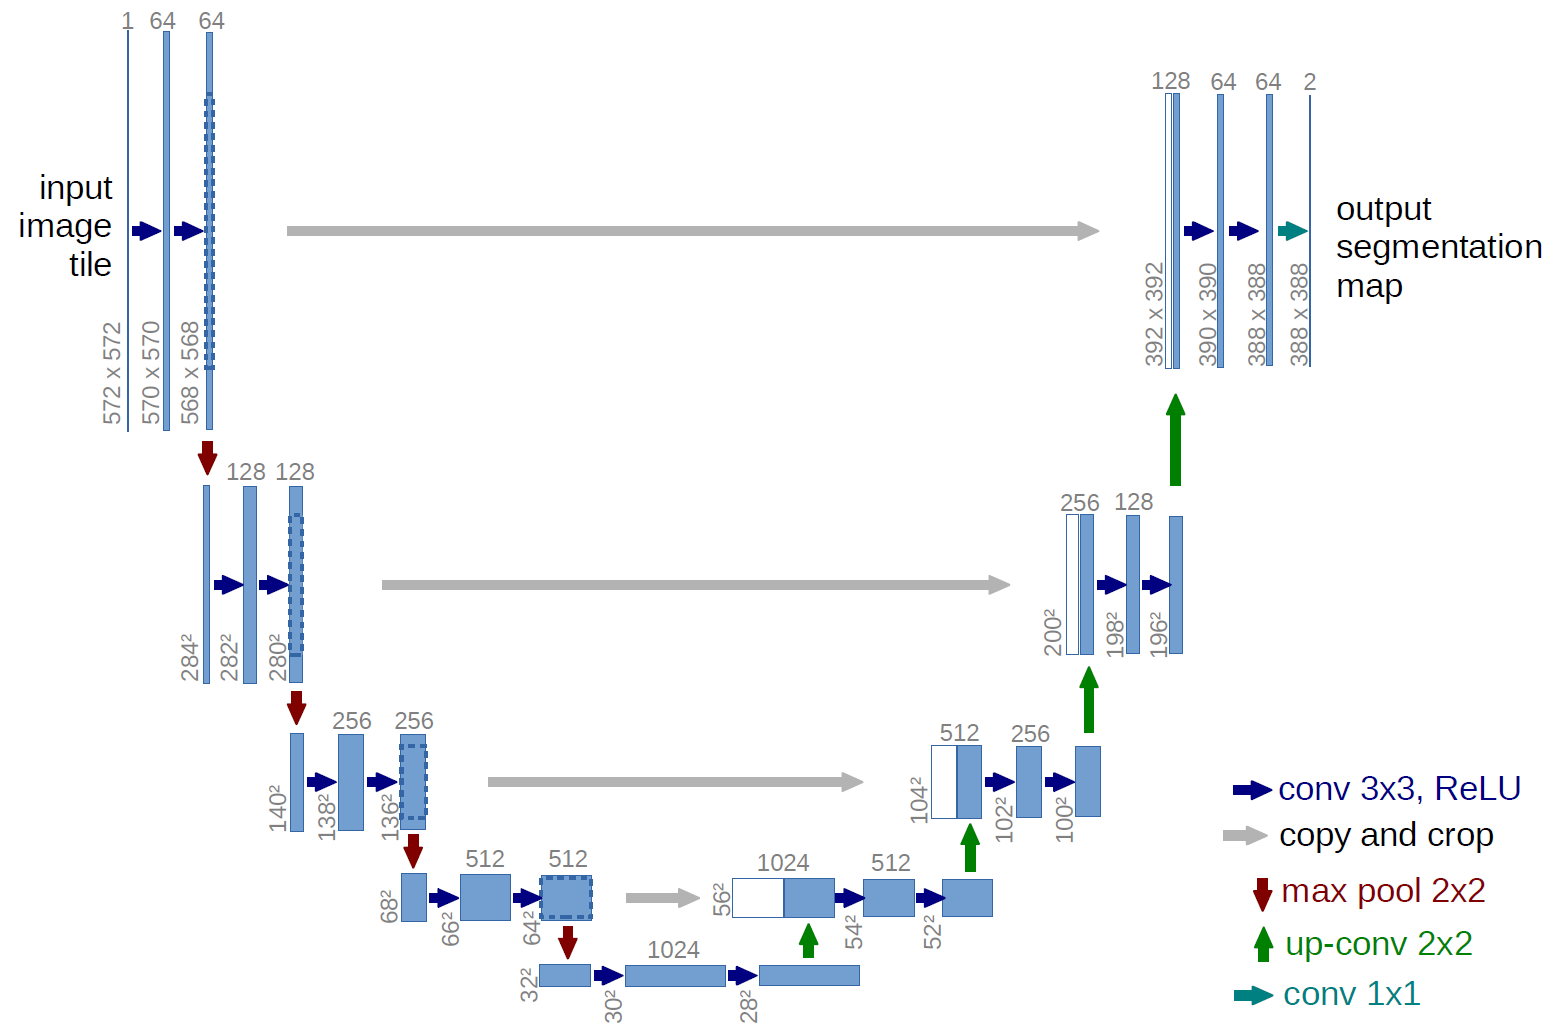
\includegraphics[width = 0.6\textheight]{figures/unet.png}
    \caption{Arquitetura de uma U-Net. Fonte: \cite{unet}.}
    \label{fig:unet}
\end{figure}

A rede consiste, basicamente, em um caminho de codificação e decodificação análogo a letra ``\textit{U}'' (veja a Figura \ref{fig:unet}). No caminho de codificação temos uma rede convolucional típica, onde há a aplicação sucessiva de convoluções, com função de ativação \textit{ReLU}, seguida de uma operação de \textit{pooling}. Por fim, o caminho de decodificação, combina características e informações espaciais, através de uma sequência de convoluções e concatenações com características, oriundas do caminho de codificação, de alta resolução \cite{iglovikov2018ternausnet}.


\subsection{Registro multiespectral}

O registro de imagens consiste, basicamente, em um método que busca uma transformação geométrica das imagens de forma a maximizar uma função de similaridade entre imagens adjacentes \cite{kumar2014survey}. Os métodos de registro de imagens podem ser classificados em pontos de controle, baseados em intensidade e métodos híbridos. Os métodos baseados em pontos de controle trabalham obtendo características bem definidas e que são compartilhadas por pares de imagens adjacentes que precisam ser registradas.

Em um contexto de imagens agrícolas obtidas por meio de veículos aéreos não tripulados, pode-se utilizar as áreas plantadas e não plantadas segmentadas como características de registro. Os métodos que se baseiam em intensidades irão considerar apenas as informações sobre a intensidade dos \textit{pixels} das imagens. Por fim, os métodos híbridos irão mesclar elementos de ambas as imagens para registro \cite{kumar2014survey}.

A ampla maioria dos métodos para registro de imagens é composto de quatro passos básicos: (1) detecção das características, (2) busca pelas características detectadas, (3) estimativa do modelo de transformação e (4) reamostragem da imagem e transformação \cite{Uchida2013ImagePA}.

Na detecção das características, objetos salientes e distintos (bordas, contornos, cantos e cruzamentos de linhas, por exemplo) são manualmente ou automaticamente detectados. Para buscar por características, a correspondência entre a imagem a ser corrigida e na imagem referência deve ser estabelecida. Diversos descritores e medidas de similaridade podem ser utilizados para obter as relações espaciais entre as características detectadas. Na estimativa do modelo de transformação, o tipo e os parâmetros das funções de mapeamento para realizar o registro entre o par de imagens será estimado. Vale ressaltar que esses parâmetros são obtidos de acordo com as características entre as duas imagens \cite{Uchida2013ImagePA}.  

Por fim, nas etapas de reamostragem e transformação, a imagem será modificada, por meio das funções de mapeamento, a fim de corrigir o deslocamento inicial entre as duas imagens. A Figura \ref{fig:etapas_registro} ilustra os quatro passos supracitados.

\begin{figure}[!ht]
    \centering
    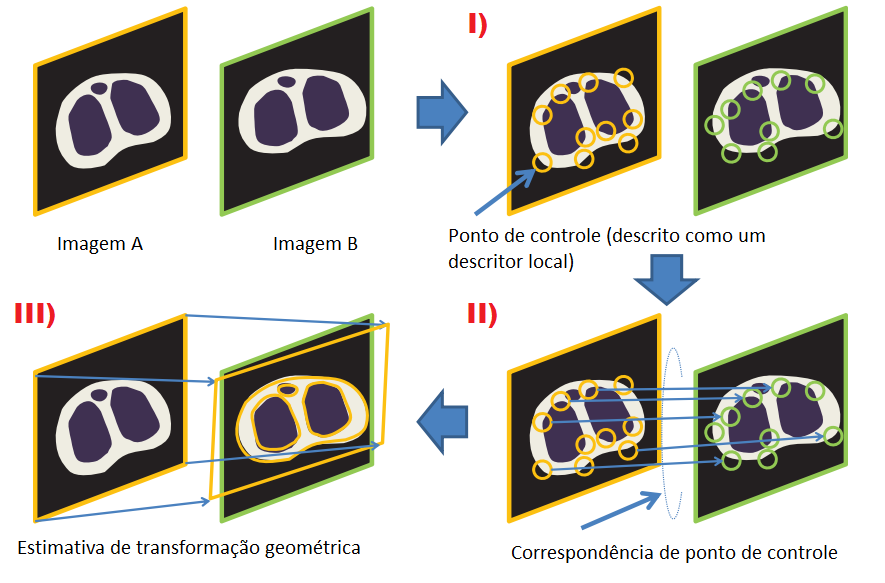
\includegraphics[width=0.75\textwidth]{figures/passos_novo.png}
    \caption{Passos necessários para o registro de imagens utilizando de pontos de controle. Em (I) tem-se a extração de \textit{features} da imagem; em (II) a combinação das características; e em (III) a função de mapeamento e a transformação da referida imagem. Fonte: \cite{Uchida2013ImagePA}.}
    \label{fig:etapas_registro}
\end{figure}

\subsubsection{Extração de características (\textit{features})}

As características (\textit{features}) podem ser entendidas como um padrão que acontece em um determinado local da imagem e distingue-se de seus vizinhos mais próximos. Em geral, tal padrão é associado a uma alteração brusca de uma (ou várias) propriedades de uma imagem (textura, cor ou intensidade, por exemplo). Os algoritmos para registro que utilizam pontos de controle encontram tais pontos analisando a magnitude e a direção das mudanças de intensidade nos vizinhos locais da imagem, com objetivo de detectar regiões, cantos e bordas \cite{kazeSuporte}.

\subsubsection{Correspondência de características (\textit{Feature matching})}

Após a extração dos pontos de controle, é preciso realizar a correspondência entre os pontos obtidos em cada uma das imagens. Duas categorias principais podem ser aplicadas para obtenção dessa correspondência: métodos exaustivos e aproximados \cite{PANTANO}.

Em um método exaustivo (força bruta, por exemplo), para cada ponto de controle obtido na primeira imagem calcula-se uma medida de distância (\textit{Hamming} para imagens binárias e \textit{Euclidiana} para as demais \cite{PANTANO}) para todos os pontos na segunda imagem. Este método busca encontrar a correspondência mais próxima para cada ponto analisado. Por mais que haja bons resultados, essa abordagem possui um alto custo computacional devido à excessiva quantidade de comparações realizadas.

Os métodos aproximados fornecem um grande ganho computacional com apenas uma pequena perda de precisão. Neste sentido, a depender da aplicação e acurácia necessária, os métodos aproximados podem ser utilizados para obtenção da correspondência entre os pontos. Dentre os algoritmos utilizados para este fim, podemos destacar: \textit{Hierarchica}, \textit{K-Means Tree} e \textit{Automatic Selection of the Optimal} \cite{PANTANO}.

\subsubsection{Construção da função de mapeamento}

Uma função de mapeamento pode ser definida matematicamente como uma função 2D, a qual mapeia as coordenadas $(x,y)$ de uma determinada imagem A para as coordenadas $(x,y)$ de uma imagem B. Dois tipos principais de função de mapeamento, Linear e Não Linear, são caracterizados pelo tipo de deformação na imagem \cite{b7}. A Figura \ref{fig:funcao_mapeamento} ilustra os tipos de transformações abordados.

\begin{figure}[!ht]
    \centering
    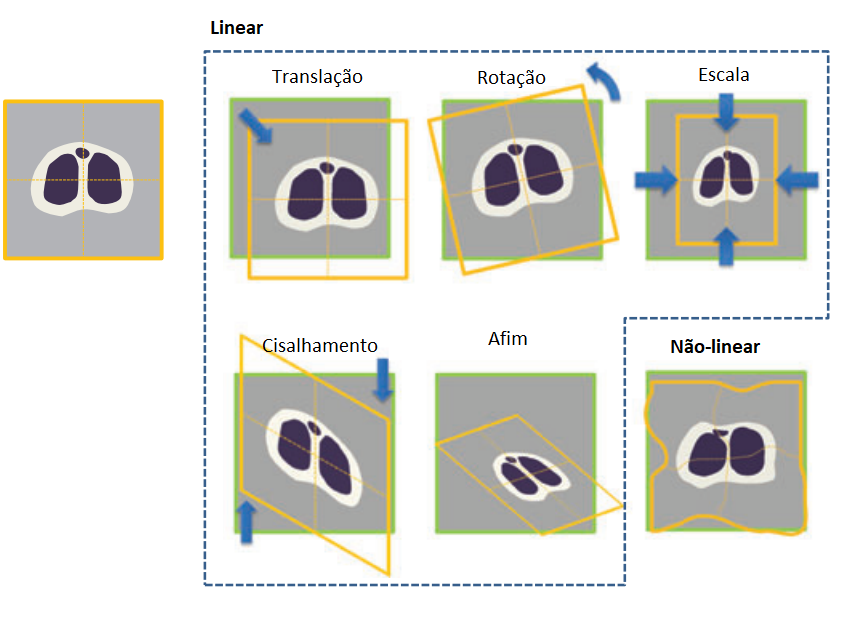
\includegraphics[width=0.75\textwidth]{figures/transformations_nova.png}
    \caption{Exemplo de transformações lineares e não lineares. Fonte: \cite{Uchida2013ImagePA}}
    \label{fig:funcao_mapeamento}
\end{figure}

\subsubsection{Transformação da imagem}

O último passo para realizar o processo de registro consiste na transformação da imagem de acordo a função de transformação obtida. Neste sentido, para transformar as imagens de acordo com uma imagem alvo, outras imagens são mapeadas conforme a referida transformação \cite{Uchida2013ImagePA}. Esse processo é ilustrado na Figura \ref{fig:transformacao_imagem}.

\begin{figure}[!ht]
    \centering
    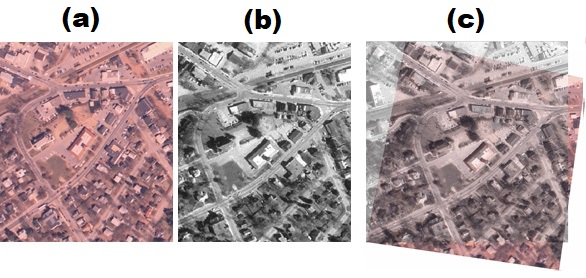
\includegraphics[width=0.5\textheight]{figures/exampleregistration.jpg}
    \caption{Exemplo de transformação de uma imagem (a) para a imagem alvo (b). O resultado da sobreposição, após a transformação, é mostrado em (c). Fonte: \cite{matlab01}}
    \label{fig:transformacao_imagem}
\end{figure}

\subsubsection{\textit{Scale Invariant Feature Transform} (SIFT)}


O algoritmo \textit{Scale Invariant Feature Transform} (SIFT) proposto por \cite{lowe} detecta pontos de controle que são descritos como características (\textit{features}) locais em uma determinada imagem. Em linhas gerais, esse algoritmo é descrito em quatro etapas: (1) Detecção de pontos de valor máximo no espaço de escala; (2) Localização de pontos de controle; (3) Atribuição de orientação; (4) Construção do vetor de características.

No primeiro estágio o algoritmo verifica a imagem, em diferentes regiões e escalas, a fim de localizar pontos de interesse invariantes à escala e orientações. Tais pontos são definidos como \textit{local scale-space} e são obtidos por meio de uma métrica denominada \textit{Difference of Gaussian (DoG)}, calculada pela subtração das diferentes escalas de Gaussianas \cite{lowe}.

Na etapa 2, localização de pontos de controle, descartam-se pontos irrelevantes, além de rejeitarmos as bordas. Pontos que possuem baixo contraste também são eliminados, de acordo com um limiar definido previamente. Em linhas gerais, para descarte destes pontos, o SIFT utiliza uma matriz \textit{Hessiana} para localizar as principais curvaturas \cite{lowe}.

Na etapa 3, o SIFT utiliza um histograma de orientação. para encontrar os descritores que são invariantes a rotação. Esse histograma parte da orientação do gradiente em cada máximo local da função \textit{DoG} (etapa 1) em uma região circunvizinha ao ponto de controle. Na maioria das vezes, essa região possui tamanho de $16 \times 16$ \textit{pixels}.

Por fim, na etapa 4, descrevemos os pontos de controle no formato de um vetor de características. Esse vetor é construído considerando a direção do ponto de controle na qual a força do gradiente é máxima. Na maioria dos casos, este vetor de características obtido pelo SIFT possui 128 elementos \cite{lowe}.

\subsubsection{\textit{Speeded-Up Robust Features} (SURF)}

Proposto por \cite{SURF}, o algoritmo SURF consiste em um detector de características (\textit{features}) que possui como base o descritor SIFT. Este algoritmo tem sido bastante utilizado em diversas áreas para a localização de características visto que seu tempo computacional é menor quando comparado com outros métodos.

O SURF utiliza a soma da \textit{wavelet2D} de \textit{Harr} em torno de um determinado ponto de interesse para a detecção de pontos de controle. A \textit{wavelet2D} de \textit{Haar} é obtida por meio de uma aproximação inteira do determinante da matriz \textit{Hessiana}, a qual extrai estruturas em forma de regiões na região onde o determinante é máximo. Deste modo, a grande melhoria no desempenho da técnica SURF está relacionada a supressão não-maximal das determinantes das matrizes Hessianas \cite{HONG20081708}.

\subsubsection{\textit{Binary Robust Invariant Scalable Keypoints} (BRISK)}

Com o objetivo de melhorar esse desempenho em relação ao SURF e ao SIFT, diferentes descritores binários foram desenvolvidos. Um desses descritores é o (BRISK). O BRISK, proposto por \cite{brisk}, é baseado no detector FAST e pode ser subdivido em: (1) padrão de amostragem, (2) compensação de orientação e (3) pares de amostragem \cite{featuresDetectors}.

O padrão de amostragem é calculado no entorno dos pontos de controle. Dessa forma, representa-se uma quantidade de pontos espalhados em diferentes círculos concêntricos, os quais são utilizados para definir se um ponto é (ou não) uma borda, sendo que tal determinação é obtida através do algoritmo \textit{Features from Accelerated Segment Test} (FAST). Posteriormente, os pontos são divididos em dois conjuntos: pontos de curta e de longa distância. A direção de cada ponto de controle é determinada através da soma do gradiente local entre os pontos pares de longa e curta distância. A fim de que haja invariância de rotação, todos os pontos são rotacionados de acordo com as orientações obtidas \cite{b3, fast}.

Por fim, as intensidades do primeiro e segundo pontos são comparadas. Caso a intensidade do primeiro ponto seja maior que a do segundo, o algoritmo retorna ``1''; senão, retorna ``0''. Desse modo, após a comparação dos 512 pontos, o descritor será determinado por um vetor de 512 \textit{bits}, sendo essa comparação entre os descritores realizada através da distância de \textit{Hamming} \cite{brisk}. 

\subsubsection{\textit{Kaze Features}}

O algoritmo \textit{Kaze} foi proposto por \cite{b5} com o objetivo de detectar características 2D dentro de um espaço de escala não linear, a fim de obter uma maior acurácia de localização e distintividade. O algoritmo \textit{Kaze}, ao contrário de outros métodos que fazem uso do método \textit{Gaussian Blurring}, realiza a filtragem de difusão não linear em conjunto com o método \textit{Additive Operator Splitting} (AOS). Vale destacar também que o algoritmo \textit{Kaze} é invariante a iluminação, escala e rotação.

A Figura \ref{fig:kaze} ilustra os pontos de controle detectados pela técnica \textit{KAZE Features} em uma imagem. Os pontos são ilustrados através de um círculo centrado neles. Assim, o raio de cada círculo representa a escala de cada ponto de controle e a linha central refere-se a orientação do ponto de controle.

\begin{figure}[!ht]
    \centering
    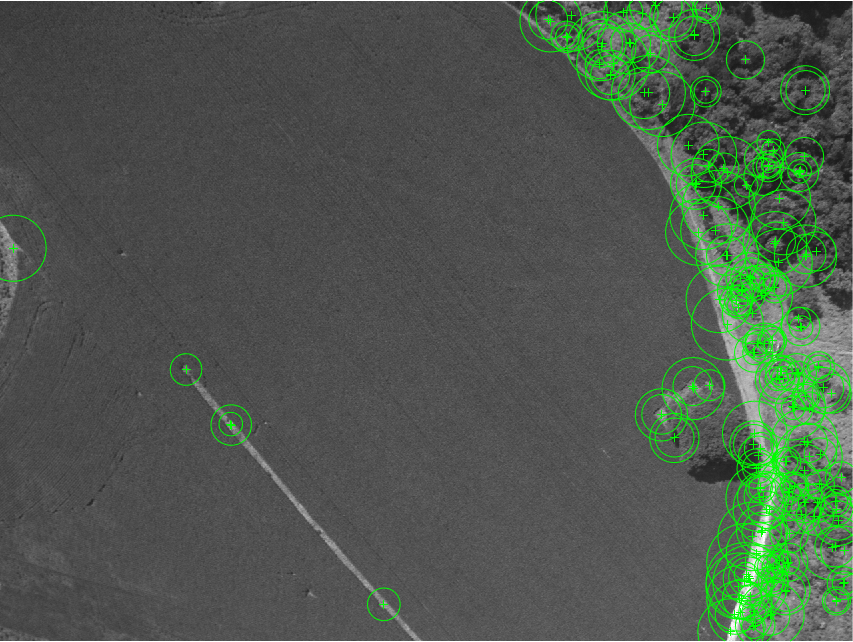
\includegraphics[width=0.5\textheight]{figures/exemplo02.png}
    \caption{Exemplo de pontos de controle, extraídos com a técnica Kaze, em uma imagem. Fonte: \cite{matlab01}.}
    \label{fig:kaze}
\end{figure}

\subsection{Métricas de avaliação}
\label{subsubsec:metricas}

Diversas técnicas têm sido utilizadas com o intuito de mensurar a qualidade do processo de registro. Duas delas, \textit{Root Mean Squared Error} (RMSE) e \textit{Back Projection Error} (BPE), serão apresentadas com maiores detalhes a seguir.

\subsubsection{\textit{Root Mean Squared Error} (RMSE)}

Segundo \cite{paula},  diferentes trabalhos já evidenciaram a importância das métricas de avaliação no processo de registro. Dentre as técnicas disponíveis, uma das mais utilizadas para essa avaliação é \textit{Root Mean Squared Error} (RMSE), a qual é obtida de acordo com a Equação \ref{eq:RMSE}:

\begin{equation}\label{eq:RMSE}
    RMSE = \sqrt{\frac{\sum_{i=1}^{N}\sum_{j=1}^{M}(P(i,j)-P'(i,j))^2}{NM}}
\end{equation}


\noindent onde $P(i,j)$ representa o \textit{pixel} na linha $i$ e coluna $j$ da imagem alinhada, $P'(i,j)$ representa o \textit{pixel} na linha $i$ e coluna $j$ da imagem registrada, $N$ representa a quantidade de \textit{pixels} da imagem alinhada e $M$ representa a quantidade de \textit{pixels} da imagem registrada. 

A partir do RMSE temos que valores menores indicam um melhor alinhamento entre duas imagens. Assim, uma das limitações da referida técnica é a necessidade de uma base previamente alinhada por um especialista para obtenção da avaliação real da performance.


\subsubsection{\textit{Back Projection Error} (BPE)}

Outra técnica que é utilizada como métrica de avaliação é a \textit{Back Projection Error} (BPE). Essa técnica representa o quão bem a localização dos pontos de controle da imagem alvo se alinham com os pontos de controle da imagem que foi registrada. Esse cálculo é realizado através da distância entre os pontos de controle da imagem registrada para os pontos de controle da imagem alvo. A Equação \ref{eq:BPE} formaliza a obtenção do BPE:

\begin{equation}\label{eq:BPE}
    BPE(I, J) = {\sum_{x\textsubscript{i},x\textsubscript{j}}d^2(X\textsubscript{I}, F\times{}X\textsubscript{J})}
\end{equation}

\noindent onde $I$ e $J$ representam, respectivamente, as imagens alvo e registrada; $d^2$ representa a métrica de distância e $F$ é a matriz de transformação. Essa técnica também apresenta a mesma limitação do RMSE, pois, quando tratamos da obtenção de resultados reais, necessita-se da utilização de uma base de dados alinhada previamente.


\subsection{Ferramentas computacionais}

Os métodos serão implementados utilizando a linguagem \textit{Python}. O \textit{Python} é uma linguagem interpretada, moderna, gratuita, possui código livre e está disponível para múltiplos sistemas operacionais \cite{perez2010python}. 

Dentre os pacotes científicos para \textit{Python}, destaca-se o \textit{NumPy}, para manipulação eficiente e de alto nível de arranjos numéricos. O \textit{SciPy} e \textit{Scikits} fornecem algoritmos de alto nível para processamento da dados científicos, incluindo processamento de imagens. O \textit{Matplotlib} é uma biblioteca poderosa para visualização de dados 2D e 3D, possibilita plotar gráficos e figuras prontas para publicação. As bibliotecas \textit{TensorFlow} e \textit{Keras} fornecem o arcabouço necessário para implementar, treinar e testar, de forma eficiente, modelos de Redes Neurais Convolucionais \cite{abadi2016tensorflow}.

\section{Trabalhos Relacionados}
\label{sec:trab_relacionados}

\subsection{Progressively trained  convolutional  neural  networks  for  deformable  image  registration}

No presente trabalho \cite{eppenhof2019progressively}, foi proposto a utilização de métodos de \textit{deep learning} para registro de imagens com distorções não-lineares como uma alternativa aos métodos tradicionais de registro. O estudo em questão é motivado pelo fato de que os métodos tradicionais não conseguem estimar grandes deslocamentos e campos de deformação complexos. 

Para o complexo cenário em questão, é necessária uma tarefa de resolução múltipla. Assim, em vez de treinar uma grande Rede Neural Convolucional (CNN) na tarefa de registro único, versões menores da rede foram inicialmente treinadas com imagens de baixa resolução e campos de deformação menos complexos. Durante o treinamento, a rede foi progressivamente expandida com camadas adicionais, que foram treinadas com dados de alta resolução. 

Os resultados mostraram que esse modo de treinamento permite que uma rede aprenda campos de deslocamentos maiores sem sacrificar a precisão do registro e que a rede resultante é menos propensa a erros de registro em comparação a executar o treinamento de toda a rede de uma só vez. Os autores também concordaram que um procedimento de treinamento progressivo leva a uma maior precisão do registro ao aprender deformações não-lineares grandes e complexas.

\subsection{\textit{Data-driven Multispectral Image Registration}}

O trabalho de \cite{yasir2018data} propõe a criação de um arcabouço computacional (\textit{framework}) para a tarefa de registro de imagens multiespectrais. Esse \textit{framework} possui como fundamento a necessidade de haver uma quantidade mínima de correspondência entre os pontos de controle entre dois canais, a fim de garantir que um baixo erro de alinhamento para que quanto maior a quantidade de pontos de controle correspondentes entre os canais, melhor será o registro.

Para obter os pontos de controle, foram utilizadas as técnicas SIFT, BRISK, SURF e \textit{Oriented Fast and Rotated BRIEF} (ORB). O referido \textit{framework} foi avaliado por meio da quantidade de pontos de controle obtidos, pelo tempo computacional e pelo \textit{Back Projection Error} (BPE). Além disso, foi avaliada a robustez do \textit{framework} em três bases de dados, sendo duas com imagens oriundas de VANTs e outra obtida através de uma plataforma fixa. Vale destacar que essas bases de dados foram escolhidas por apresentarem uma considerável variedade de distorções diferentes.

Em linhas gerais, o \textit{framework} apresentado no trabalho consiste na construção de um grafo completo, no qual os nós do grafo são os canais a serem registrados e os pesos dos pontos de controle de quantidade obtidos pelos algoritmos entre os canais. Desse modo, ao utilizar o algoritmo de Kruskal constrói-se uma árvore geradora máxima. 

A fim de localizar o canal a ser utilizado como alvo para os outros alinhamentos, a árvore geradora máxima é transformada novamente em um grafo colocando peso em suas arestas. Posteriormente, o algoritmo Floyd-Warshall é aplicado para que se obtenha os caminhos mais curtos entre os vértices. Assim, o nó com a menor soma de distâncias de si mesmo para todos os outros nós adjacentes é selecionado como o canal destino para o trabalho de registro. Neste cenário podem haver nós intermediários no processo, sendo esta uma das principais vantagens do \textit{framework} proposto. A Figura \ref{fig:framework} apresenta um esquema geral do \textit{framework} abordado no trabalho.

\begin{figure}[!ht]
    \centering
    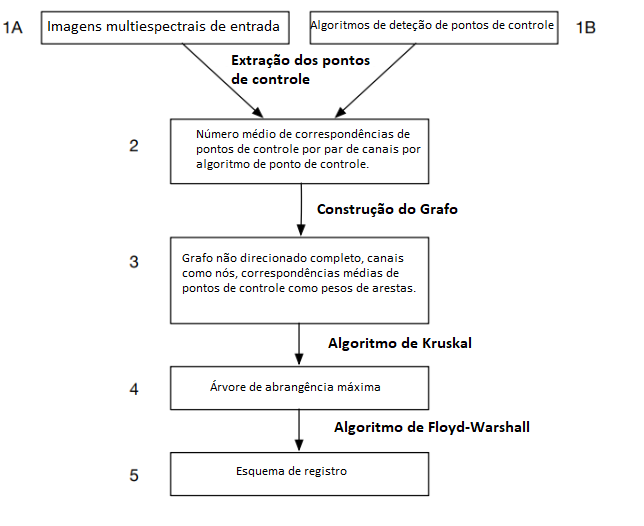
\includegraphics[width=0.6\textheight]{figures/framework_novo.png}
    \caption{\textit{Framework} proposto no trabalho. Fonte \cite{yasir2018data}.}
    \label{fig:framework}
\end{figure}


\subsection{Detection of control points for UAV-Multispectral sensed data registration through the combining of feature descriptors}

O trabalho de \cite{junior2019detection} mostra que a popularização da utilização de Veículos Aéreos Não Tripulados, concomitante ao desenvolvimento de novos sensores, permitiram a aquisição e utilização de imagens multi e hiperespectrais na agricultura de precisão. Por outro lado, a execução do processo de registro de imagens consiste em uma tarefa complexa, devido à falta de características da imagens entre os vários espectros e as distorções criadas pela utilização dos VANTS no processo de aquisição. Diante disso, o objetivo deste trabalho foi avaliar diferentes técnicas para obtenção de pontos de controle em imagens multiespectrais de plantações de soja obtidas por VANTS e investigar se a combinação de características oriundas de diferentes técnicas geram melhores resultados do que quando as referidas técnicas são utilizadas individualmente. 

O trabalho avaliou três algoritmos de detecção com características distintas (KAZE, MEF e BRISK) e suas combinações. Os resultados do trabalho evidenciam que a técnicas KAZE possui os melhores resultados.

Em linhas gerais, os trabalhos de \cite{junior2019detection} e \cite{dias2020uav}, embora não abordem transformações não lineares, contribuirão consideravelmente para este. Primeiramente, levando em consideração que para realizar o co-registro é preciso selecionar uma banda para chama-la de ``fixa'', ou, em outras palavras, as demais bandas devem se alinhar em direção a essa banda ``fixa''. \cite{dias2020uav} demonstra que o melhor canal para se denominar ``fixo'' é o \textit{verde}. Além disso \cite{junior2019detection, dias2020uav} contribui de forma substancial para a definição e formulação das distorções entre bandas em imagens multiespectrais obtidas por VANTs.



\section{Metodologia} 
\label{sec:metodologia}

Este projeto consiste em quatro etapas principais, conforme ilustrado na Figura \ref{fig:metodologia}: (1) pré-processamento; (2) detecção das distorções presentes nas imagens e a respectiva correção dessas distorções; (3) realização do registro multiespectral; e (4) avaliação dos resultados.


\begin{figure}[!ht]
    \centering
    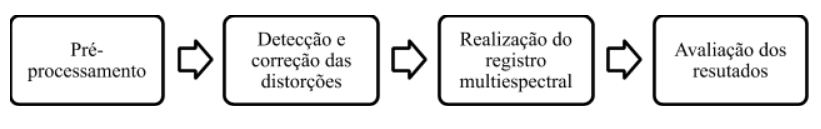
\includegraphics[width=0.85\textwidth]{figures/metodologia.png}
    \caption{Fluxo de trabalho de um sistema para registro de imagens multiespectrais.}
    \label{fig:metodologia}
\end{figure}



\subsection{Pré-processamento} 

Nessa etapa serão aplicadas diversas técnicas de pré-processamento, as quais fomentam as etapas posteriores. Pretende-se também avaliar o grau de influência dessas técnicas no aumento da acurácia do co-registro multiespectral.

\subsection{Detecção e correção das distorções}

A partir de técnicas de \textit{deep learning}, em especial as Redes Neurais Convolucionais (CNN), espera-se detectar e classificar as distorções presentes em cada imagem analisada, além do grau dessas distorções detectadas.

Ainda com o auxílio de técnicas de \textit{deep learning}, além das tradicionais, espera-se corrigir a(s) distorção(es) detectada(s), a fim de potencializar a etapa posterior de realização do co-registro multiespectral.

\subsection{Realização do registro multiespectral}

Nessa etapa será realizado, através de técnicas tradicionais e emergentes, o registro entre as bandas das imagens em questão. O detalhamento das técnicas a serem utilizadas, suas vantagens e desvantagens, foram detalhadas na seção de Revisão da Literatura.

\subsection{Avaliação dos resultados}

A fim de avaliar o co-registro multiespectral, serão utilizados, principalmente, o \textit{Root Mean Squared Error} (RMSE) e o \textit{Back Projection Error} (BPE), os quais foram discutidas na seção \ref{subsubsec:metricas}. 

\section{Resultados esperados} 
\label{sec:resultados}

Ao fim do projeto, espera-se quatro resultados principais:

\begin{enumerate}
    \item \textbf{Caracterização do problema de co-registro multiespectral de imagens para agricultura de precisão obtidas por VANTs.} 
    
    Espera-se caracterizar e definir o problema de co-registro multiespectral de imagens para agricultura de precisão, obtidas por VANTs. Atualmente, a literatura que sumarize o problema na AP não é muito vasta. Ainda assim, o trabalho de \cite{junior2019detection} se destaca e servirá como uma das bases para este estudo.
    
    \item \textbf{Detecção de distorções não-lineares em imagens oriundas do voo de VANTs para a aplicação em questão.} 
    
    Espera-se detectar as distorções não-lineares, a fim de fomentar a correção e futuro co-registro. Esse processo de detecção de qual distorção, bem como o seu grau, facilitará os processos posteriores.
    
    \item \textbf{Correção das distorções detectadas na etapa 2}.
    
    Esta etapa refere-se ao processo de correção das referidas distorções, com o objetivo de potencializar o processo de registro das referidas imagens.
    
    \item \textbf{Maior precisão no co-registro multiespectral de imagens para agricultura de precisão obtidas por VANTs.} 
    
    Por fim, espera-se conseguir uma maior acurácia no alinhamento multiespectral entre bandas de imagens obtidas por VANTs. Conforme já mencionado neste projeto, há diversas abordagens para o co-registro multiespectral, entretanto, todos os métodos apresentam determinadas limitações, o que pode, eventualmente, não gerar ótimos resultados de alinhamos. Dessa maneira, há a proposta de formalização de um método com objetivo de aumentar a precisão do alinhamento multiespectral de imagens aéreas obtidas por VANTs.
    
\end{enumerate}


\section{Cronograma de Execução} 
\label{sec:cronograma}


Até o presente momento, foram realizados estudos sobre as principais técnicas de co-registro de imagens e classificação de distorções oriundas do voo do VANT. 

A Tabela \ref{tab:cronograma}, onde cada linha representa uma atividade e cada coluna um mês (\textbf{a partir de novembro de 2020}), apresenta o cronograma de execução completo com as etapas inerentes ao trabalho.


\begin{table}[!ht]
\caption{Cronograma de atividades}
\centering

\begin{tabular}{c|c|c|c|c|c|c|c|c|c|}
\cline{2-10}
 & \multicolumn{2}{c|}{2020} & \multicolumn{7}{c|}{2021} \\ \cline{2-10} 
 & Nov. & Dez. & Jan. & Fev. & Mar. & Abril & Mai. & Jun. & Jul. \\ \hline
\multicolumn{1}{|c|}{Atividade 1} & x & x &  &  &  &  &  &  &  \\ \hline
\multicolumn{1}{|c|}{Atividade 2} &  & x &  &  &  &  &  &  &  \\ \hline
\multicolumn{1}{|c|}{Atividade 3} &  & x & x &  &  &  &  &  &  \\ \hline
\multicolumn{1}{|c|}{Atividade 4} &  &  & x & x &  &  &  &  &  \\ \hline
\multicolumn{1}{|c|}{Atividade 5} &  &  &  & x & x &  &  &  &  \\ \hline
\multicolumn{1}{|c|}{Atividade 6} &  &  &  & x & x & x &  &  &  \\ \hline
\multicolumn{1}{|c|}{Atividade 7} &  &  &  &  &  & x & x & x & x \\ \hline
\multicolumn{1}{|c|}{Atividade 8} &  &  &  &  &  &  & x & x & x \\ \hline
\end{tabular}
\label{tab:cronograma}
\end{table}


\begin{itemize}

    \item \textbf{Atividade 1:} Revisão bibliográfica sobre técnicas de detecção e classificação das principais distorções oriundas de imagens capturadas por VANTs, bem como de técnicas de co-registro de imagens multiespectrais.
    \item \textbf{Atividade 2:} Avaliação dos algoritmos e métodos levantados.
    \item \textbf{Atividade 3:} Aplicação de técnicas para detecção e classificação das principais distorções analisadas neste trabalho.
    \item \textbf{Atividade 4:} Aplicação de técnicas de co-registro selecionadas.
    \item \textbf{Atividade 5:} Seleção dos principais métodos/técnicas aderentes ao trabalho.
    \item \textbf{Atividade 6:} Avaliação dos resultados gerais.
    \item \textbf{Atividade 7:} Escrita e submissão de artigos científicos para congressos e/ou periódicos da área.
    \item \textbf{Atividade 8:} Escrita e defesa da dissertação.
    
\end{itemize}

\noindent Uberlândia, 10 de novembro de 2020.

\bibliographystyle{sbc} % sbc
\bibliography{bibliography}
\end{document}